\documentclass[a4paper,11pt]{article}
\usepackage[margin=2.5cm]{geometry} % Make more reasonable margins in document
\usepackage[parfill]{parskip}  % Remove LaTeX indents, and add interparagraph space
\usepackage[utf8]{inputenc}
\usepackage[english]{babel}

\usepackage{enumitem} % Enumerations met letters in de plaats van cijfers

%%%%%%%%%%%%
%%% MATH %%%
%%%%%%%%%%%%
\usepackage{mathtools}
\usepackage{amssymb}
\usepackage[output-decimal-marker={,}]{siunitx}
\newcommand\Log[1]{ \mathop{{}^{#1}\mathrm{log}} }
\DeclarePairedDelimiterX{\norm}[1]{\lVert}{\rVert}{#1}

% https://tex.stackexchange.com/questions/94032/fancy-tables-in-latex
\usepackage[table]{xcolor}
\usepackage{booktabs}

\usepackage[utf8]{inputenc}
\usepackage{pdfpages}

%Visuals
\usepackage{graphicx}
\usepackage{subcaption}
\usepackage[colorlinks,allcolors=violet]{hyperref}
\usepackage{url}
\usepackage[T1]{fontenc}
\usepackage{lmodern} 
\usepackage{algorithm}
\floatname{algorithm}{Algoritme}
\usepackage{algorithmic}
\usepackage{courier}
\usepackage{wrapfig}
\usepackage[export]{adjustbox}
\usepackage{wasysym}

%Figures
\usepackage{pgfplots}
\pgfplotsset{compat=newest}
%% the following commands are needed for some matlab2tikz features
\usetikzlibrary{plotmarks}
\usetikzlibrary{arrows.meta}
\usepgfplotslibrary{patchplots}
\usepackage{grffile}
\usepackage{amsmath}
\usepackage{caption}
\usepackage{float}
\usepackage{cleveref}
\usepackage{multirow}
\usepackage{titlesec}
\usepackage{listings}

\usepackage{multicol}
\usepackage{tikz}
\lstset{
	language=Matlab,
	%    basicstyle={\ttfamily \small},
	basicstyle={\ttfamily \small},
	%    keywordstyle=\underline,
	numberstyle={\footnotesize},
	%    morekeywords={ones,mod,isprime,inline,unique,factor,@},
	%    flexiblecolumns=false,
	%    emph={gamma,beta},
	%    emphstyle=,
	columns=fullflexible,
	%    columns=flexible,
	%    commentstyle={\slshape},
	%    commentstyle={\normalfont},
	commentstyle={\ttfamily},
	stringstyle={\ttfamily \bfseries},
	showstringspaces=false,
	%    indent=1em,
	%    xleftmargin=0.5em,
	breaklines=false,
	%    frame={l},
	captionpos={t},
	upquote=true, % such that we can copy-paste the code...
	%    mathescape=true,
	%    frame=single,     % boxed in a single line
	%    frame=L,          % double line on the left
	%    frame=l,          % single line on the left
}

\newcommand*\circled[1]{\tikz[baseline=(char.base)]{
            \node[shape=circle,draw,inner sep=0.1pt] (char) {#1};}}
\newcommand{\note}[1]{{\colorbox{yellow!40!white}{#1}}}
\titleformat{\section}
{\normalfont\Large\bfseries}{\boxed{\text{Assignment \thesection}}}{1em}{}

\setlength{\pdfpageheight}{11in}


\title{Nonlinear Systems \\[1ex]
    \Large \textsc{Assignments}}
\author{Elias Wils}
\date{\today}

\begin{document}

\maketitle
\newpage
\tableofcontents

\newpage
\section{Stability of equilibrium points and bifurcations}    
\subsection{A simple population model}
\paragraph{Question 1}\: The position and number of equilibrium points depends on the value of $\alpha$ and $\beta$.
In \Cref{tbeq1} the different possible cases are listed together with information about the equilibrium points.
When looking at the graph of $\dot{N}$ against $N$, a negative parabola can be observed, intersecting the $N$-axis in two points.
When solving the quadratic equation for $\dot{N}=0$ with $\alpha$ and $\beta$ as unknown parameters, expressions shown in (1) and \eqref{eqN2} for
the equilibrium points ensue.
\begin{align}
	N_1 &= 0\\
	N_2 &= \frac{K(\alpha-\beta)}{\alpha}
	\label{eqN2}
\end{align}
\begin{table}[H]
	\centering
	\begin{tabular}{|c|c|c|}
	\hline
	$\alpha<\beta$ & $\alpha>\beta$ & $\alpha=\beta$\\
	\hline
	$N_1$ is stable (\CIRCLE) & $N_1$ is unstable (\Circle) & $N_1=N_2$\\
	$N_2$ is unstable (\Circle) & $N_2$ is stable (\CIRCLE) & half stable equilibrium point (\RIGHTcircle)\\
	\hline
	\end{tabular}
	\captionsetup{width=0.9\textwidth}
	\caption{Summary of the characteristics of the equilibrium points for different cases of $\alpha$ and $\beta$. }
	\label{tbeq1}
\end{table}
The type of bifurcation that occurs here is called transcritical. A qualitative representation of this bifurcation can be seen in 
\Cref{fig:trbif}, with the different cases in the same order as in \Cref{tbeq1}. Here the x-axis represents $N$, and the 
y-axis represents $\dot{N}$
\begin{figure}[H]
	\centering
	\makebox[\textwidth][c]{
	\begin{subfigure}{0.45\linewidth}
		\centering
		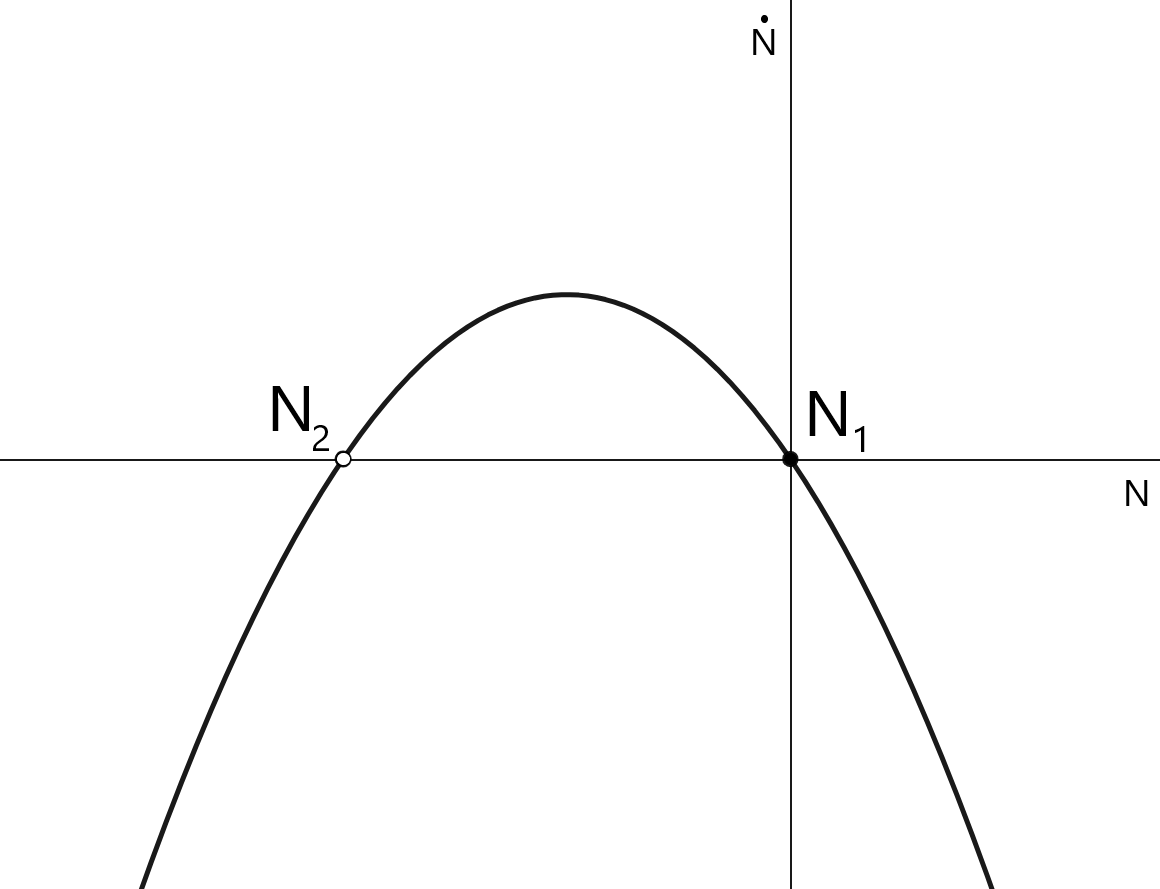
\includegraphics[width=\textwidth]{altb.png}
		\caption{$\alpha<\beta$}
	\end{subfigure}\hfill
	\begin{subfigure}{0.45\linewidth}
		\centering
		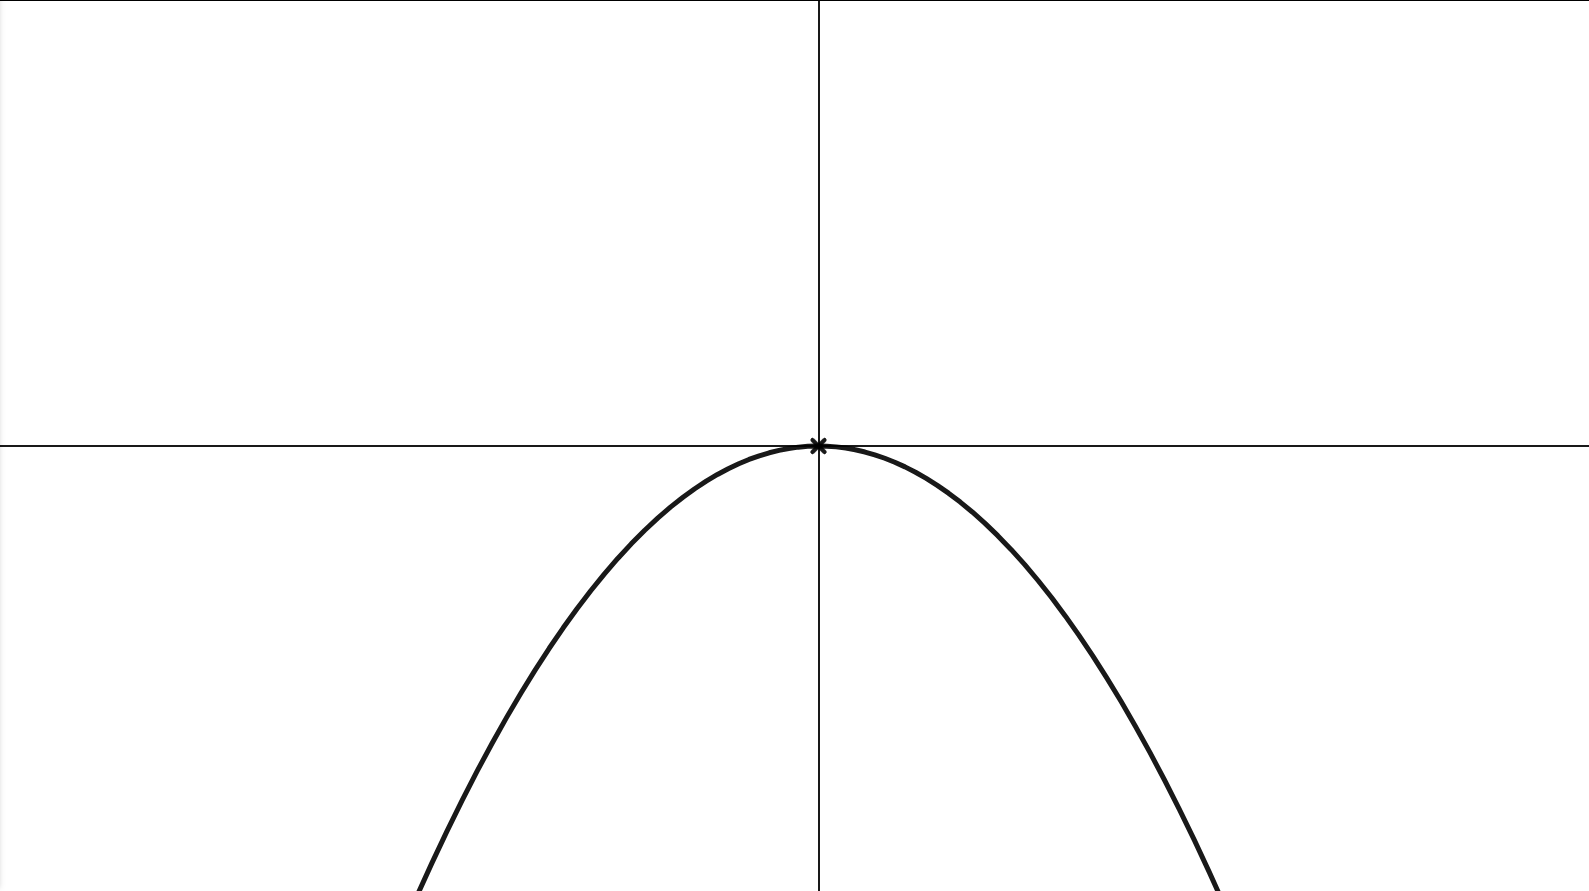
\includegraphics[width=\textwidth]{aisb.png}
		\caption{$\alpha=\beta$}
	\end{subfigure}
	\begin{subfigure}{0.45\linewidth}
		\centering
		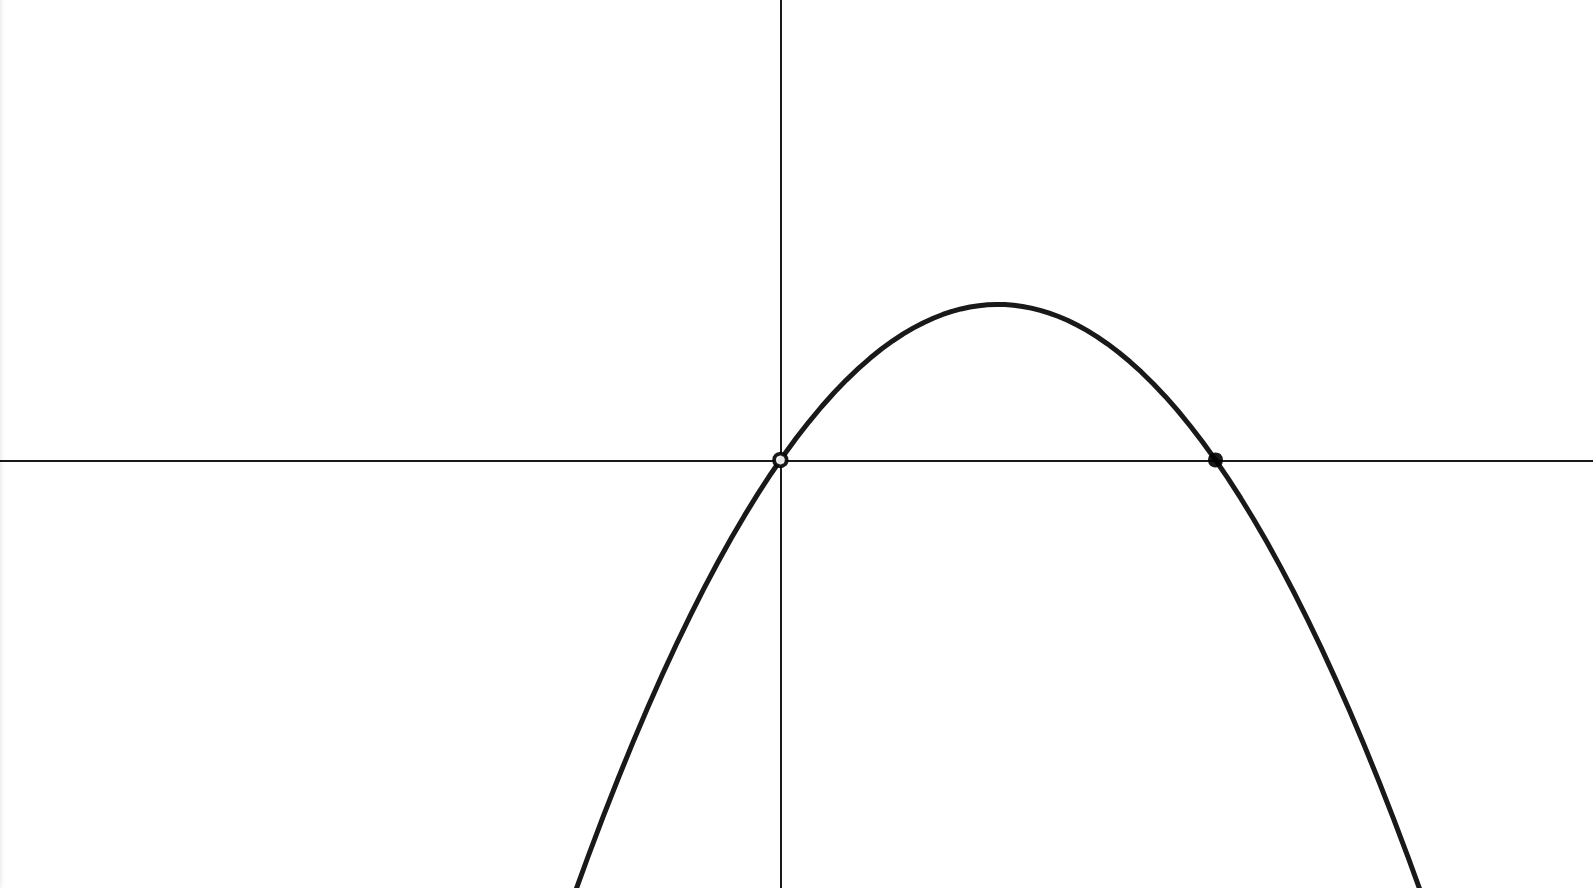
\includegraphics[width=\textwidth]{agtb.png}
		\caption{$\alpha>\beta$}
	\end{subfigure}
	}
	\caption{Qualitative plot of $\dot{N}$ against N for the different cases for $\alpha$ and $\beta$.}
	\label{fig:trbif}
\end{figure}
\paragraph{Question 2}\: For the practical example described here, the solution for $t\rightarrow\inf$ will converge to one 
of the equilibrium points. As $\alpha>\beta$, the second case in \Cref{tbeq1} is applicable. The only stable equilibrium point
is $N_2=\frac{K(\alpha-\beta)}{\alpha}=10\:470\:086$. Thus, with the parameters declared in the assignment text,
the number of inhabitants will converge towards the stable equilibrium $N_2$, which is $10\:470\:086$ here, as 
$t\rightarrow\infty$.\\

\subsection{Gene control model}
\paragraph{Question 1}\: When taking the repression rate $r=0$, only one fixed point is visible. 
The system equations become:
\begin{equation*}
	\begin{cases}
		 \dot{x}=\frac{\alpha_1}{2}-x\\
		 \dot{y}=\frac{\alpha_2}{2}-y
	\end{cases}
\end{equation*}
The only fixed point is $\left(\frac{\alpha_1}{2}, \frac{\alpha_2}{2}\right)$. We can classify fixed points
of a 2-dimensional system by analyzing the system matrix. As this system is nonlinear The Jacobian is taken 
as an approximation of this system matrix. Then the system becomes linear and an appropriate stability analysis
can be done. Below the computations are first done for the general case, whereafter $r=0$ is filled in.
The Jacobian of this nonlinear system becomes:
\begin{equation*}
	J=
	\begin{bmatrix}
		-1 & -\frac{\alpha_1ry^{r-1}}{(y^r+1)^2}\\
		-\frac{\alpha_2rx^{r-1}}{(x^r+1)^2} & -1
	\end{bmatrix}=
	\begin{bmatrix}
		-1 & 0\\
		0 & -1
	\end{bmatrix}
\end{equation*}
The trace $\tau$ of this matrix is $-2$ and the determinant $\Delta$ is:
\begin{equation*}
	\Delta=1-\frac{\alpha_1\alpha_2r^2x^{r-1}y^{r-1}}{(x^r+1)^2(y^r+1)^2}=1
\end{equation*}
In the Strogatz book there is summarized how fixed points can be classified through
$\tau$ and $\Delta$. Here $\tau<0$ and $\Delta>0$, and $\tau^2-4\Delta=0$. This means that this fixed
point is a \textbf{degenerate node}. It lies on the border between nodes and spirals, and it means that the 
eigenspace corresponding to the only eigenvalue is one-dimensional.
\paragraph{Question 2}\: $\alpha_1=\alpha_2=2$ and $r>0$.
\vspace{-5	mm}
\paragraph{i.}\: An obvious fixed point here is $(1, 1)$, and this is verified by \texttt{PPLANE},
as seen in \Cref{fig:pp1}, where a value of $r=1$ is used. 
\vspace{-5mm}
\paragraph{ii.}\: When studying the stability, there can again be made use of the Jacobian derived earlier and
fill in the given values for the parameters and $(x,y)=(1,1)$.
\begin{equation*}
	J=
	\begin{bmatrix}
		-1 & -\frac{\alpha_1ry^{r-1}}{(y^r+1)^2}\\
		-\frac{\alpha_2rx^{r-1}}{(x^r+1)^2} & -1
	\end{bmatrix}=
	\begin{bmatrix}
		-1 & -\frac{r}{2}\\
		-\frac{r}{2} & -1
	\end{bmatrix}
\end{equation*}
The expression for the determinant then becomes:
\begin{equation*}
	\Delta=1-\frac{\alpha_1\alpha_2r^2x^{r-1}y^{r-1}}{(x^r+1)^2(y^r+1)^2}=1-\frac{r^2}{4}
\end{equation*}
The trace $\tau$ stays -2. For $0< r< 2$, $\tau<0$ and $\Delta>0$ just as in Question 1.
However, now $\tau^2-4\Delta>0$, so for this range for $r$ $(1,1)$ is a stable node.\\ The special case
where $r=0$ is worked out in Question 1, then $(1,1)$ is a degenerate node. \\
Then also $r=2$ deviates from the rest. The determinant $\Delta$ then becomes zero, which means that one
of the eigenvalues is zero as the Jacobian becomes a matrix of just $-1$s. When $r$ exceeds 2, the determinant
$\Delta$ becomes negative, which means a saddle node is established.\\
These findings are summarized in \Cref{tbeq2}.
\begin{table}[H]
	\centering
	\begin{tabular}{|c|c|c|c|}
	\hline
	$r=0$ & $0<r<2$ & $r=2$ & $r>2$\\
	\hline
	$\tau=-2<0$ & $\tau=-2<0$ & $\tau=-2<0$ & $\tau=-2<0$\\
	$\Delta=1>0$ & $\Delta\in(0,1)>0$ & $\Delta=0$ & $\Delta<0$\\
	$\tau^2-4\Delta=0$ & $\tau^2-4\Delta\in(0,4)>0$ & $\tau^2-4\Delta=4>0$ & $/$\\
	degenerate node & stable node & stable line of nodes & saddle node\\
	\hline
	\end{tabular}
	\captionsetup{width=0.9\textwidth}
	\caption{Summary of the characteristics of the fixed point $(1,1)$ for $0\leq r\leq2$.}
	\label{tbeq2}
\end{table}
\vspace{-5mm}
The phase portraits for these cases are shown in \Cref{fig:pp1}, as requested in \textbf{iv}.
\vspace{-3mm}
\paragraph{iii.}\: There can be noticed that a bifurcation occurs when $r$ crosses the value 2. This bifurcation is a 
supercritical pitchfork bifurcation, because when $r>2$, a pair of stable equilibrium points appear symmetrically w.r.t. the fixed point $(1,1)$.
This fixed point $(1,1)$ is stable when $0<r<2$ and becomes unstable when $r>2$ as it becomes a saddle node.
These types of bifurcations occur in systems where there is some sort of symmetry present, as is the case here.
The two system equations are exactly the same, apart from the fact that $x$ and $y$ are interchanged. This also causes the 
Jacobian to be almost symmetrical, apart from the interchanged $x$ and $y$ again.\\
This is also seen when computing the phase plane numerically with \texttt{PPLANE}. Once $r$ exceeds 2, 
two more fixed points arise symmetrical w.r.t. the original fixed point $(1,1)$.

\paragraph{iv.}\: The phase portraits for the different cases of $r$ listed in \Cref{tbeq2} are shown in \Cref{fig:pp1}.
\begin{figure}[H]
	\centering
	\makebox[\textwidth][c]{
	\begin{subfigure}[b]{0.5\textwidth}
		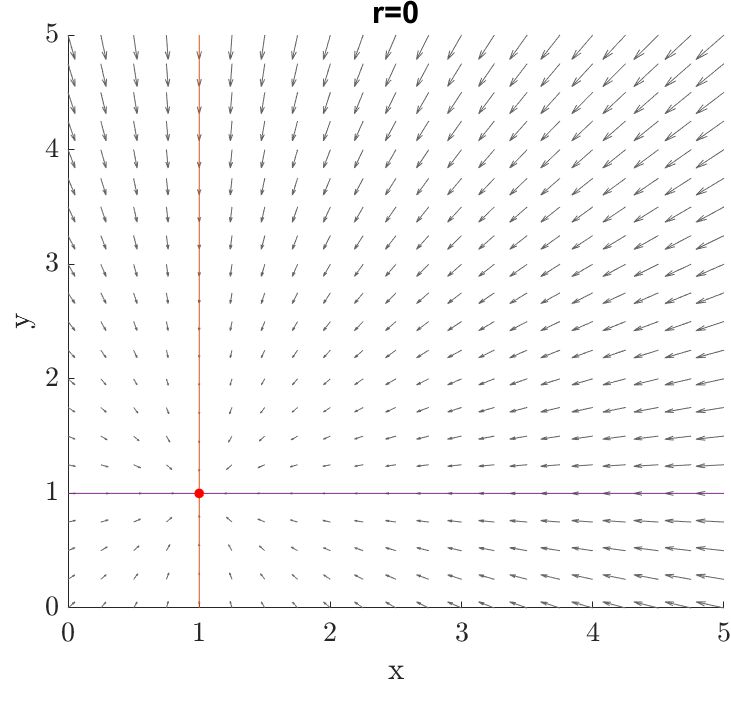
\includegraphics[width=\textwidth]{r0.png}
		\caption{Phase portrait for $r=0$.}
		\label{fig:r0} 
	\end{subfigure}

	\begin{subfigure}[b]{0.5\textwidth}
		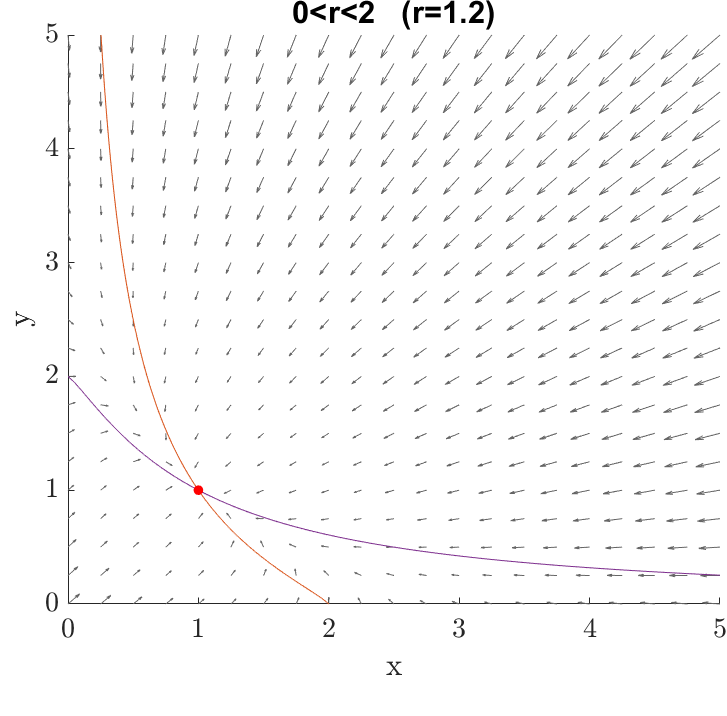
\includegraphics[width=\textwidth]{0r2.png}
		\caption{Phase portrait for $r=1.2$.}
		\label{fig:0r2}
	\end{subfigure}
	}
	\makebox[\textwidth][c]{
	\begin{subfigure}[b]{0.5\textwidth}
		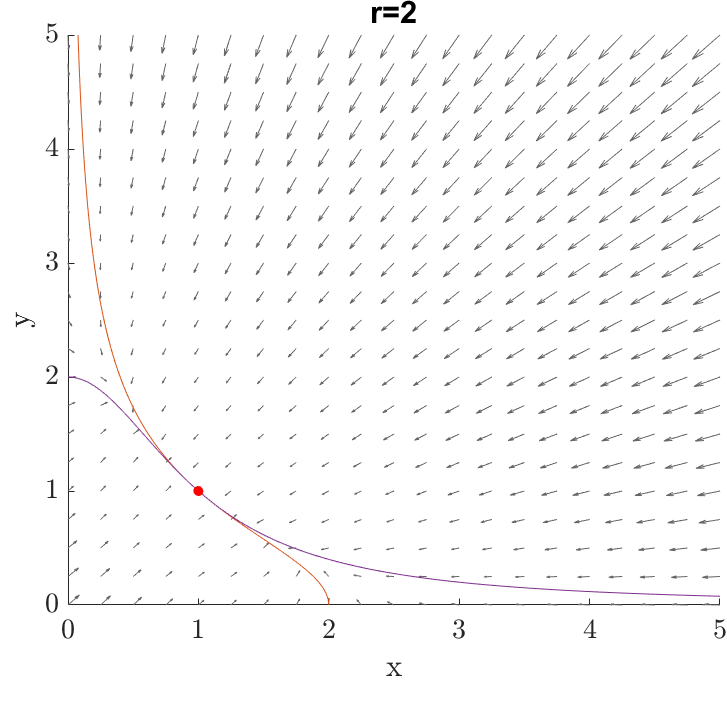
\includegraphics[width=\textwidth]{r2}
		\caption{Phase portrait for $r=2$.}
		\label{fig:r2} 
		\end{subfigure}
		
		\begin{subfigure}[b]{0.5\textwidth}
		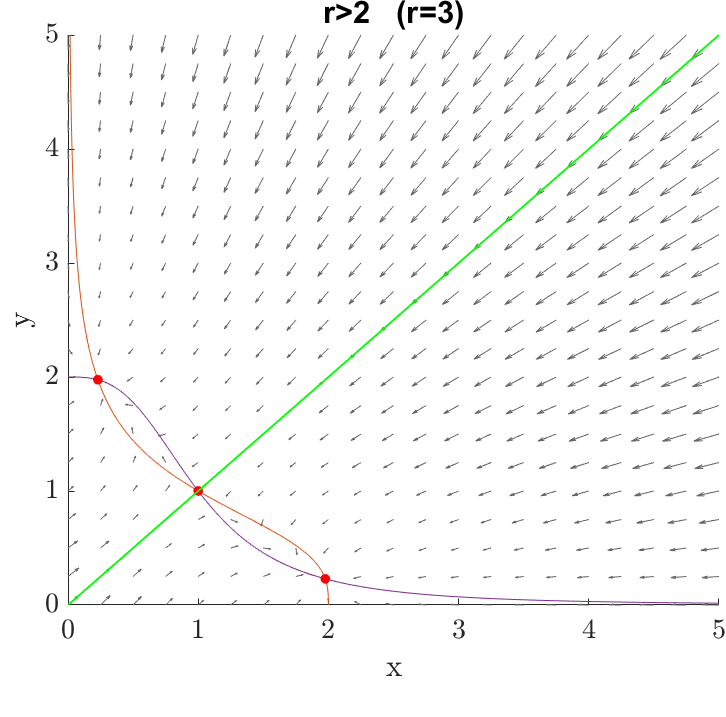
\includegraphics[width=\textwidth]{rgt2.png}
		\caption{Phase portrait for $r=3$.}
		\label{fig:rgt2}
		\end{subfigure}
	}
	\label{fig:pp1}
	\vspace{-3mm}
	\caption{Phase portraits of the given system for the qualitatively different phase portraits when varying $r$.}
\end{figure}
The bifurcation that occurs here is a supercritical pitchfork bifurcation, and a qualitative sketch of the bifurcation diagram of
either $x$ or $y$ is shown in \Cref{fig:bif}.
\begin{figure}[H]
	\centering
	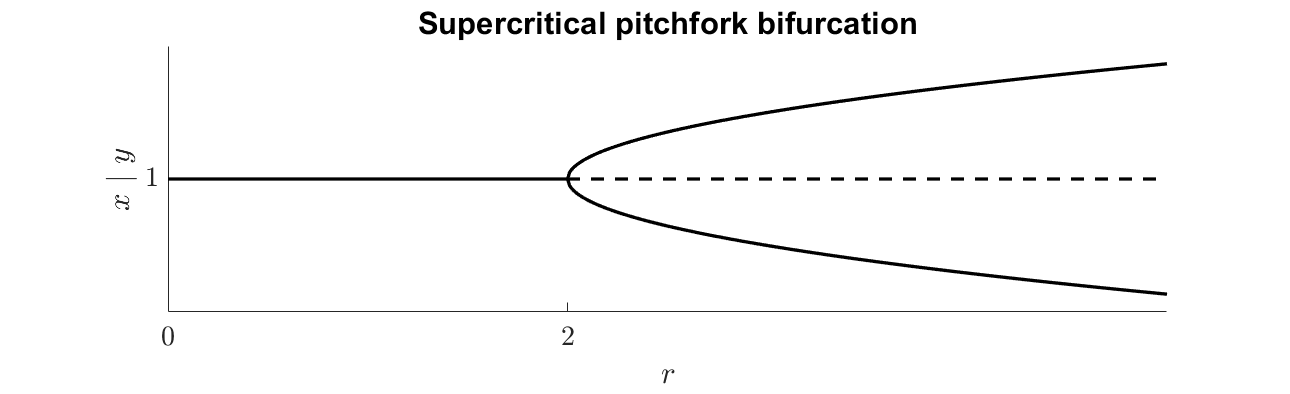
\includegraphics[width=1.1\textwidth]{suppit.png}
	\caption{Qualitative bifurcation diagram of the supercritical pitchfork bifurcation.}
	\label{fig:bif} 
\end{figure}

\newpage
\section{Imperfect bifurcations}
\subsection{Gene control revisited}
The accurate bifurcation diagram using \texttt{COCO} can be found in \Cref{fig:bif1}. The diagram for both
$x$ and $y$ in function of $r$ is plotted, as the diagram 3-dimensional.
\begin{figure}[H]
	\centering
	\makebox[\textwidth][c]{
	\begin{subfigure}[b]{0.5\textwidth}
		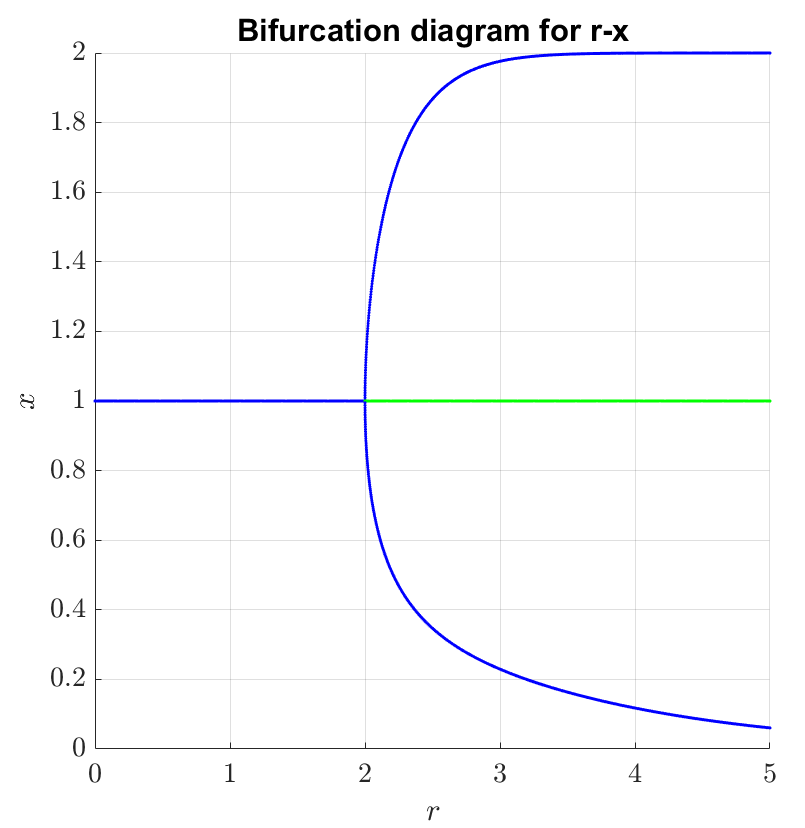
\includegraphics[width=\textwidth]{bif1x.png}
		\caption{Pitchfork for $r$ and $x$.}
		\label{fig:bif1x} 
	\end{subfigure}\hfill

	\begin{subfigure}[b]{0.503\textwidth}
		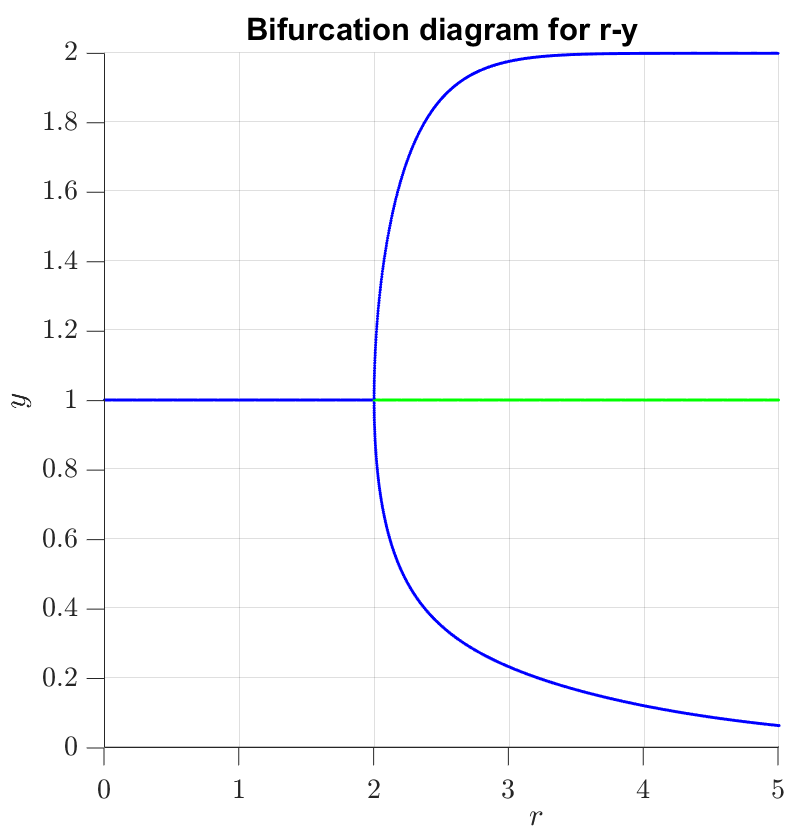
\includegraphics[width=\textwidth]{bif1y.png}
		\caption{Pitchfork for $r$ and $y$.}
		\label{fig:bif1y}
	\end{subfigure}
	}
	\label{fig:bif1}
	\caption{Bifurcation diagram of the supercritical pitchfork bifurcation in both $x$ and $y$, obtained with \texttt{COCO}.}
\end{figure}
The blue line represents the stable equilibrium points, while the green line represents the 
saddle nodes that become present when $r>2$. The supercritical pitchfork bifurcation can be noticed very well.

\subsection{Imperfect bifurcations}
\paragraph{Question 1}\: The bifurcation diagram of the given equilibrium equation can be plotted for different values of $r$ 
in function of $h$ and $x$. When $-1\leq r\leq0$, the bifurcation diagram has no turning points present, and consists of one 
continuous curve of stable equilibrium points.\\
When $0<r\leq1$, two turning points arise in a symmetric fashion, together with a branch of unstable equilibrium points
in the middle. \\
The transition between those two cases arises when $r=0$. Then the point $(x,h)=(0,0)$ is a non-generic turning point (or degenerate fold).
This non-generic turning point is indicated by a red dot in \Cref{fig:bifhxr0}.
The bifurcation diagrams of these cases are shown in \Cref{fig:bifhx}.

\begin{figure}[H]
	\centering
	\makebox[\textwidth][c]{
	\begin{subfigure}{0.43\linewidth}
		\centering
		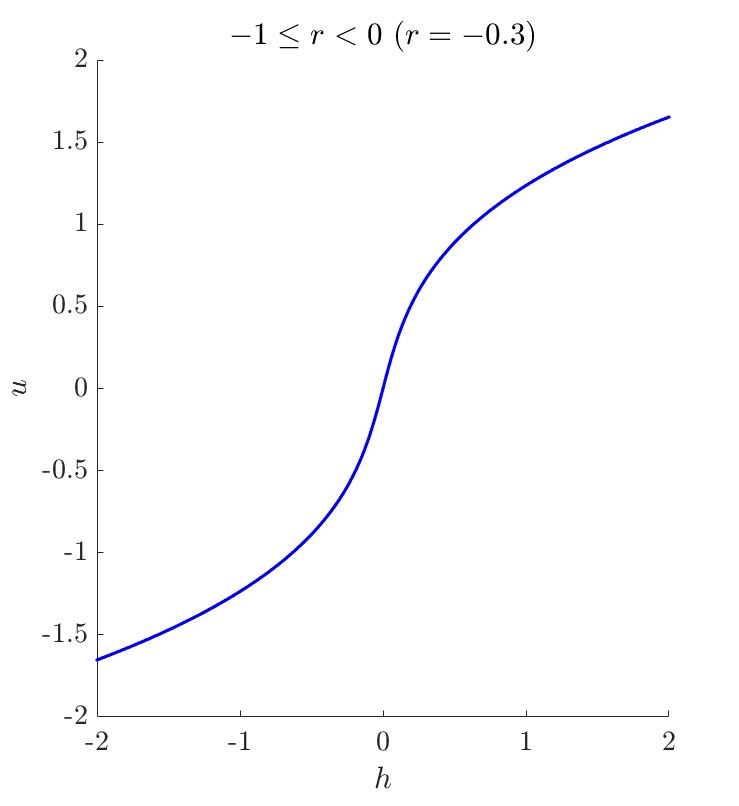
\includegraphics[width=\textwidth]{bifhxr-1.png}
		\caption{$r\in[-1,0)$, here $r=-0.3$}
	\end{subfigure}\hfill
	\begin{subfigure}{0.43\linewidth}
		\centering
		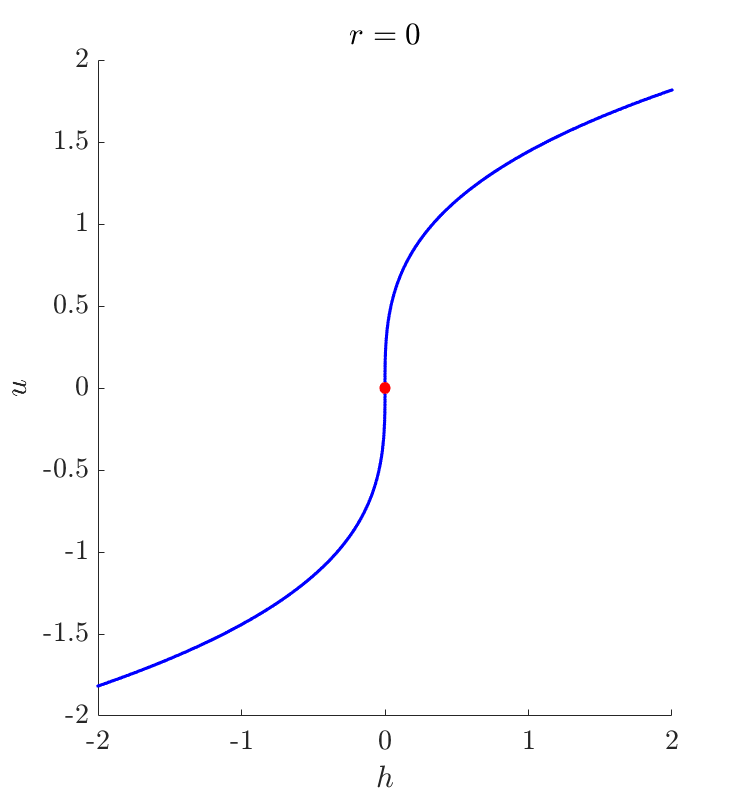
\includegraphics[width=\textwidth]{bifhxr0.png}
		\caption{$r=0$}
		\label{fig:bifhxr0}
	\end{subfigure}
	\begin{subfigure}{0.43\linewidth}
		\centering
		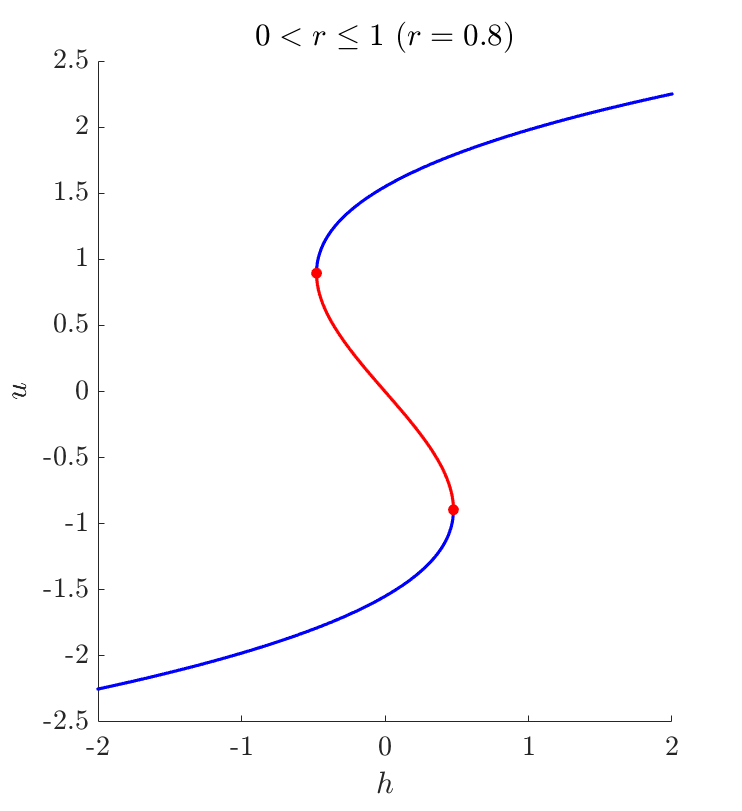
\includegraphics[width=\textwidth]{bifhxr1.png}
		\caption{$r\in(0,1]$, here $r=0.8$.}
	\end{subfigure}
	}
	\caption{Bifurcation diagrams in function of $h$ for different values of $r$.}
	\label{fig:bifhx}
	\vspace{-4mm}
\end{figure}

\paragraph{Question 2}\: Then also the bifurcation diagram can be plotted for different values of $h$ 
in function of $r$ and $x$. The diagram is plotted in \Cref{fig:bifrx} for three values of $h$: $-0.1$, 0 and 1.\\
When $h=0$, a regular supercritical pitchfork can be seen.\\ When h is decreased under zero, for example $-0.1$, 
The pitchfork is separated into two separate smooth curves, one with stable equilibrium points, and one with
a turning point.\\
When $h>0$, for example 0.1, the pitchfork decomposes again, but this time in the opposite direction.
Again \\
The parameter $h$ serves as an \textit{imperfection parameter}, as it removes the symmetry of the pitchfork bifurcation
as $h\neq0$.
This imperfection parameter $h$ can also be seen as a perturbation of a model. In real life problems 
the model that is constructed doesn't always correspond exactly to reality.
$h$ can be interpreted as an additive perturbation, thus there can be explained why fixed points arise
and disappear when a model is perturbed.

\begin{figure}[H]
	\centering
	\vspace{-1mm}
	\makebox[\textwidth][c]{
	\begin{subfigure}{0.43\linewidth}
		\centering
		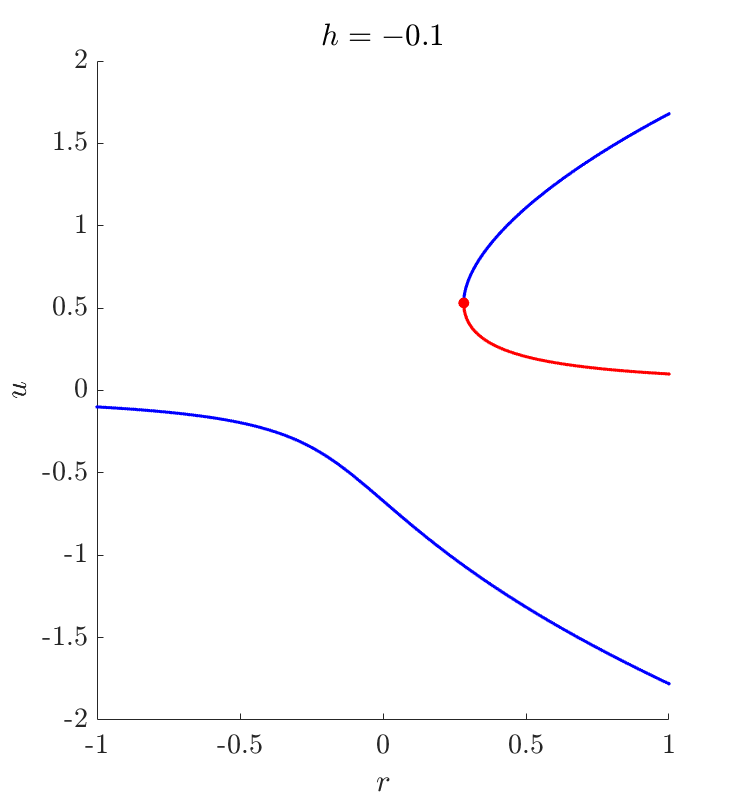
\includegraphics[width=\textwidth]{bifrxh-1.png}
		\caption{$h=-0.1$}
	\end{subfigure}\hfill
	\begin{subfigure}{0.43\linewidth}
		\centering
		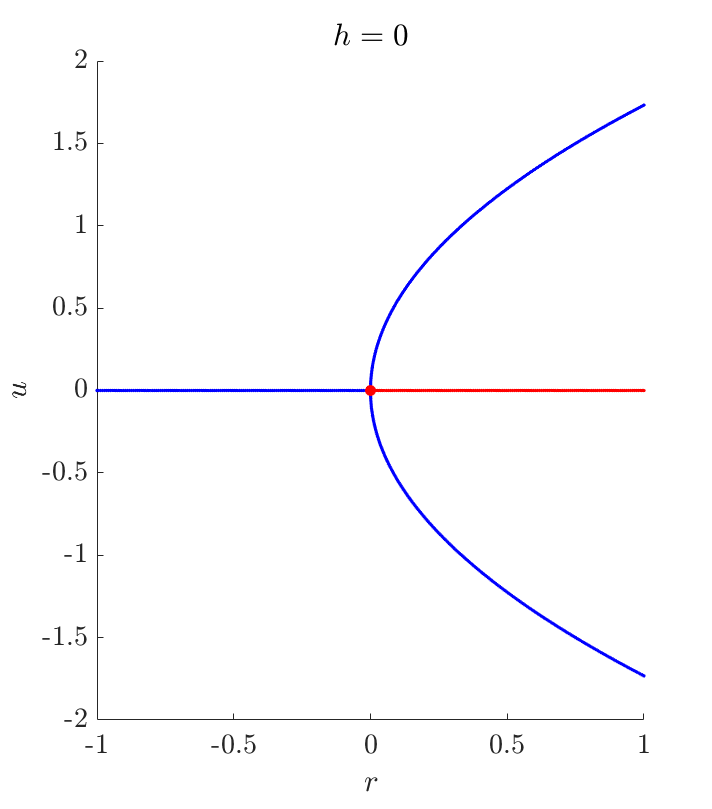
\includegraphics[width=\textwidth]{bifrxh0.png}
		\caption{$h=0$}
		\label{fig:bifrxh0}
	\end{subfigure}
	\begin{subfigure}{0.43\linewidth}
		\centering
		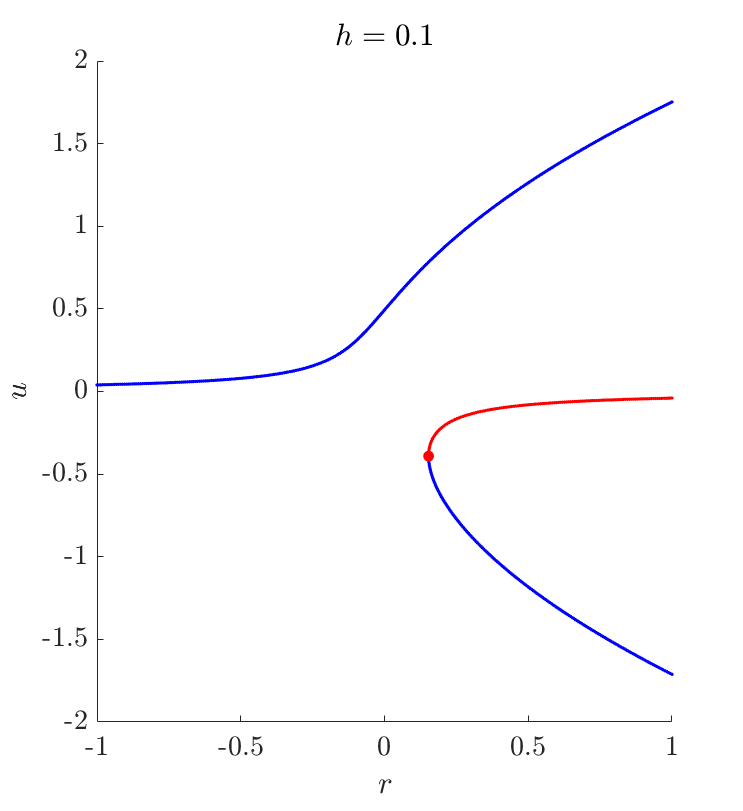
\includegraphics[width=\textwidth]{bifrxh1.png}
		\caption{$h=0.1$}
	\end{subfigure}
	}
	\caption{Bifurcation diagrams in function of $r$ for different values of $h$.}
	\label{fig:bifrx}
\end{figure}

\paragraph{Question 3}\: The fold curve was determined using \texttt{COCO}, and the result is shown in \Cref{fig:foldc}.
The projections on the $(u,r)$, $(u,h)$ and $(r,h)$ plane is plotted.
\begin{figure}[H]
	\centering
	\makebox[\textwidth][c]{
	\begin{subfigure}{0.43\linewidth}
		\centering
		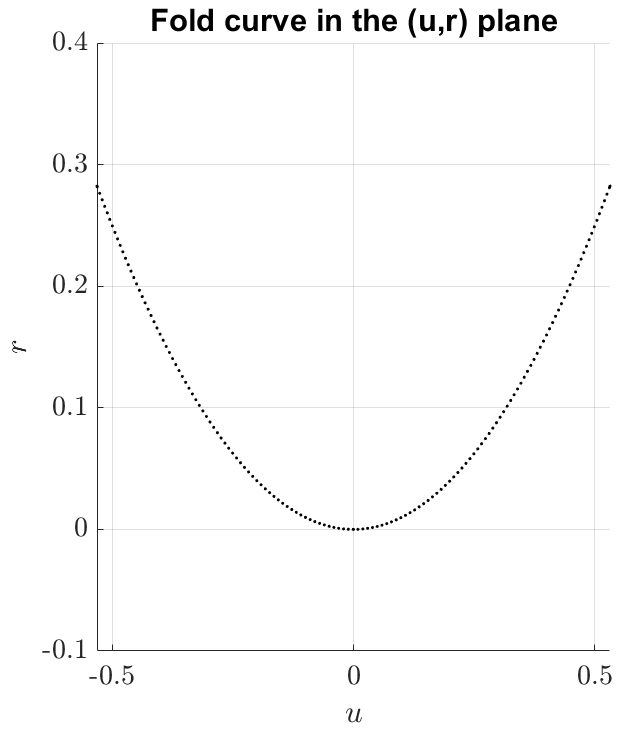
\includegraphics[width=\textwidth]{foldur.png}
		\caption{$(u,r)$ plane}
	\end{subfigure}\hfill
	\begin{subfigure}{0.43\linewidth}
		\centering
		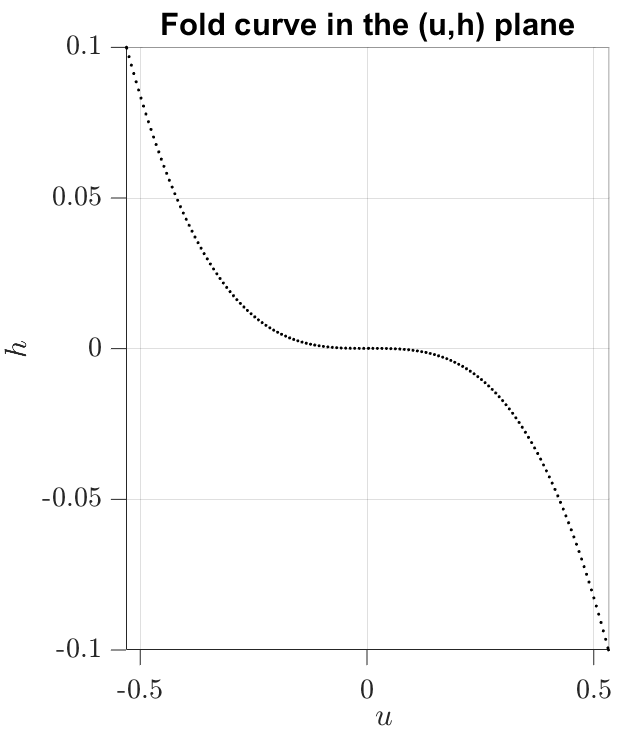
\includegraphics[width=\textwidth]{folduh.png}
		\caption{$(u,h)$ plane}
	\end{subfigure}
	\begin{subfigure}{0.43\linewidth}
		\centering
		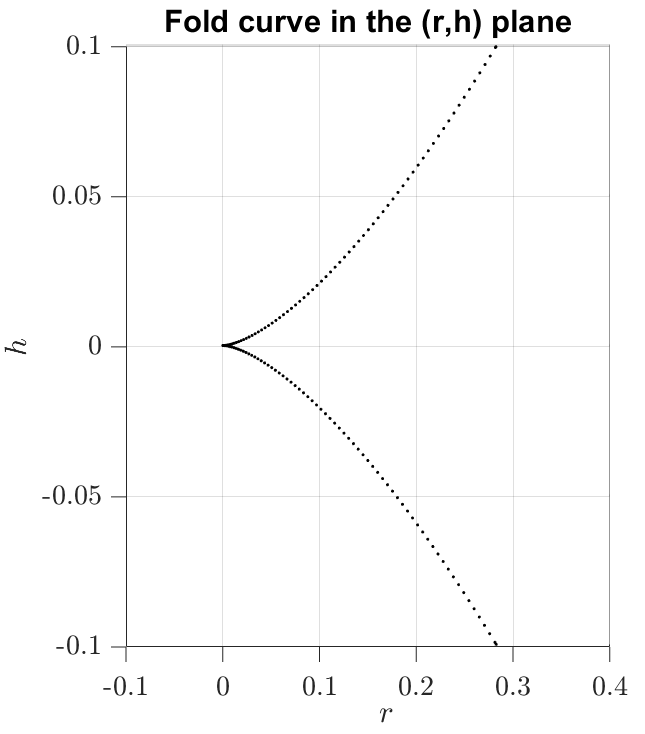
\includegraphics[width=\textwidth]{foldrh.png}
		\caption{$(r,h)$ plane}
		\label{fig:foldcrh}
	\end{subfigure}
	}
	\caption{Fold curve projected on the 2-dimensional $(u,r)$, $(u,h)$ and $(r,h)$ planes.}
	\label{fig:foldc}
\end{figure}
These three curves are the projections of the cusp catastrophe surface. When looking at the $(r,h)$ projection,
there can be noticed that when the curve is crossed, a \textit{catastrophe} occurs and the behaviour of the system
changes abruptly.\\
The correlation of the $(r,h)$ mapping (\Cref{fig:foldcrh}) with the bifurcation plots (\Cref{fig:bifhx} and \Cref{fig:bifrx})
is clearly visible. The point $(r,h)=(0,0)$ can be seen as a transition point, and it is also the starting point
of the fold curve in \Cref{fig:foldcrh}. In this point the system transitions from having one turning point, to having
three. The symmetry of this fold curve can also be seen through the plot at Question 1 (\Cref{fig:bifhx}), where 
two additional turning points arise when $h>0$ and drift away from each other in symmetrical fashion. When studying the evolution
of these fixed points and mapping it to the $(r,h)$ plane, the plot from \Cref{fig:foldcrh} can be constructed.\\
Also the other two mappings to the $(u,r)$ and $(u,h)$ plane can be constructed from looking at the evolution 
of the turning points in the plots from Question 1 and 2 (\Cref{fig:bifhx} and \Cref{fig:bifrx})

\paragraph{Question 4}\: For this question the influence of four continuation parameters within \texttt{COCO} was studied for 
a point very close to the cusp point. Namely the the bifurcation diagram in function of $r$ is asked for small 
negative values of $h$, so right at the point where the pitchfork breaks into two branches.
The bifurcation diagrams are depicted below in \Cref{fig:bifh}.
\begin{figure}[H]
	\centering
	\makebox[\textwidth][c]{
	\begin{subfigure}[b]{0.5\textwidth}
		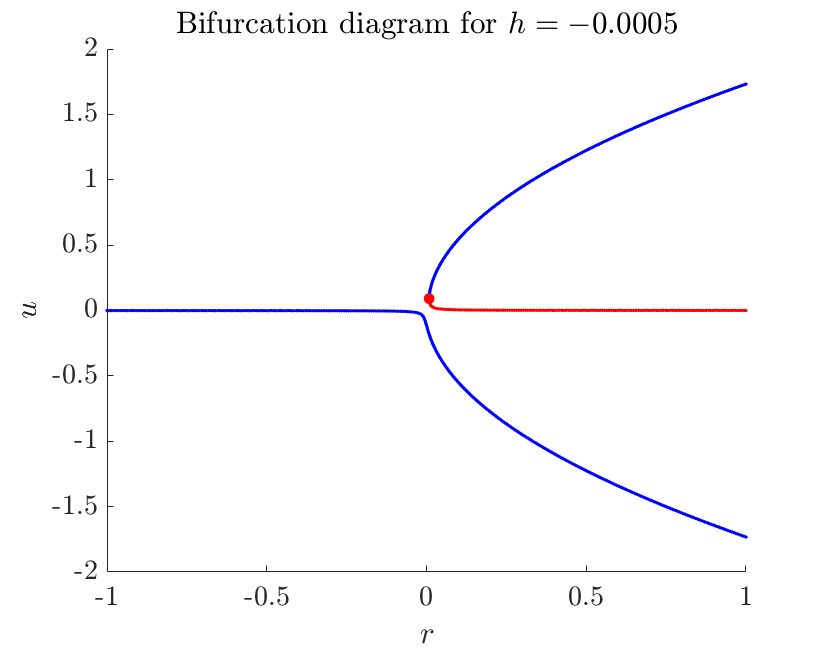
\includegraphics[width=\textwidth]{h5.png}
		\caption{\texttt{h\_max=0.05}}
	\end{subfigure}\hfill

	\begin{subfigure}[b]{0.5\textwidth}
		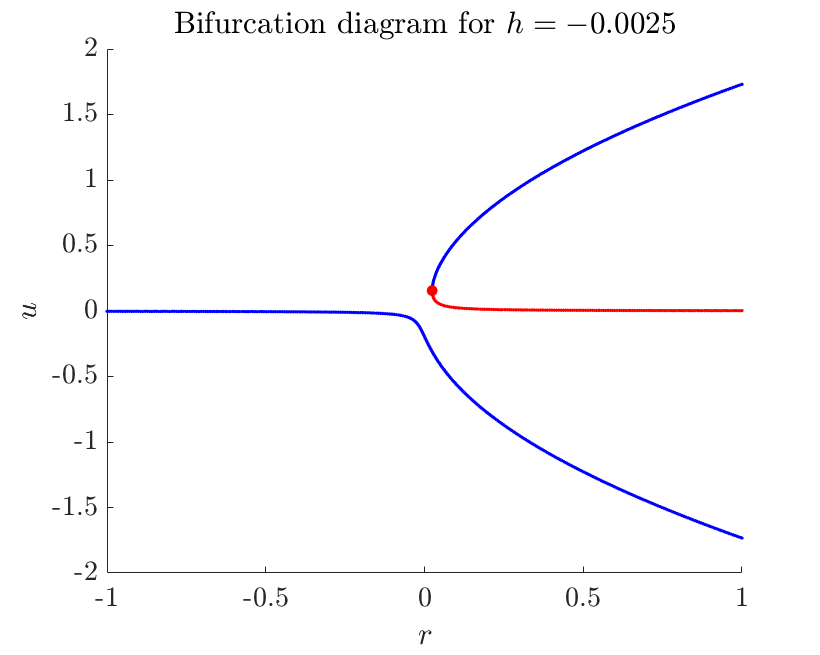
\includegraphics[width=\textwidth]{h25.png}
		\caption{\texttt{h\_max=0.05}}
	\end{subfigure}
	}
	\caption{Bifurcation diagrams in function of $r$ for $h=-0.0005$ and $h=-0.0025$, obtained with \texttt{COCO}.}
	\label{fig:bifh}
\end{figure}
These parameters are listed below, together with a short explanation and their influence on the result. Then also
a few plots are shown, which demonstrate the effects of these parameters when they are not set properly.\\
\begin{itemize}
	\item \texttt{h\_min}\: This is the minimum step size (incrementation of the parameter) for the continuation, in the course
	slides denoted as $\Delta\lambda$. This parameter allows to set a lower bound on this step size, so not more points are computed
	than necessary. \\When this bound is too large, an unwanted branch switch may occur. This is illustrated in \Cref{fig:bs}.
	For small values of $h$, this has a higher chance of happening, so the step size has to be small enough.
	\item \texttt{h\_max}\: This is the maximum step size $\Delta\lambda$. \\This parameter thus functions as an upper bound, and also
	needs to be small enough, otherwise the unwanted branch switch (\Cref{fig:bs}) can occur. For small $h$ it needs to be chosen small
	enough as well, but has to be larger than \texttt{h\_min} of course.
	\item \texttt{cont - ItMX}\: This parameter determines the maximum number of iterations during continuation. In other words,
	this parameter determines how many steps on a branch are taken at maximum. \\When a small step size is chosen, this parameter
	needs to be large enough, otherwise the branch may not be fully computed in the desired interval. In \Cref{fig:steps} is shown
	what happens when the parameter is too small.
	\item \texttt{corr - ItMX}\: This also functions as an upper bound on the number of iterations, but this time during the Newton
	correction of the gradient when a step is taken. If this parameter is chosen too small, the solution will be computed very inaccurately and will
	mostly look very different from the real solution.
	Luckily Newton doesn't need many iterations in our case (2-3), so a value 10 is more than enough. In general there probably won't be needed
	a lot of iterations because of the quadratic convergence of the Newton iteration.
\end{itemize}
\begin{figure}[H]
	\centering
	\makebox[\textwidth][c]{
	\begin{subfigure}[b]{0.5\textwidth}
		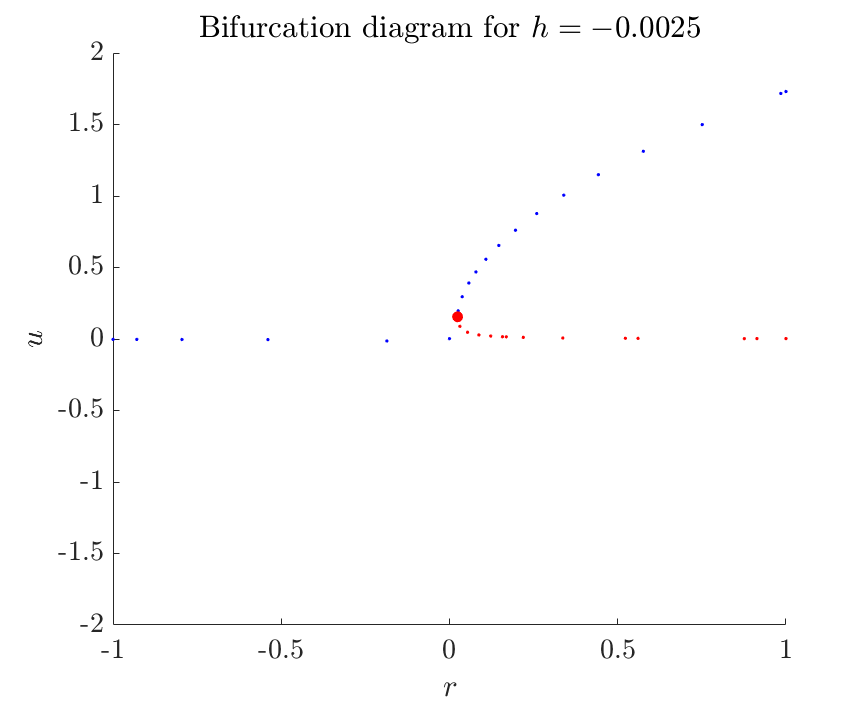
\includegraphics[width=\textwidth]{bs.png}
		\captionsetup{width=0.9\textwidth}
		\caption{Branch switch - step size $\Delta\lambda$ too large (\texttt{h\_max=0.05}).}
		\label{fig:bs}
	\end{subfigure}\hfill

	\begin{subfigure}[b]{0.5\textwidth}
		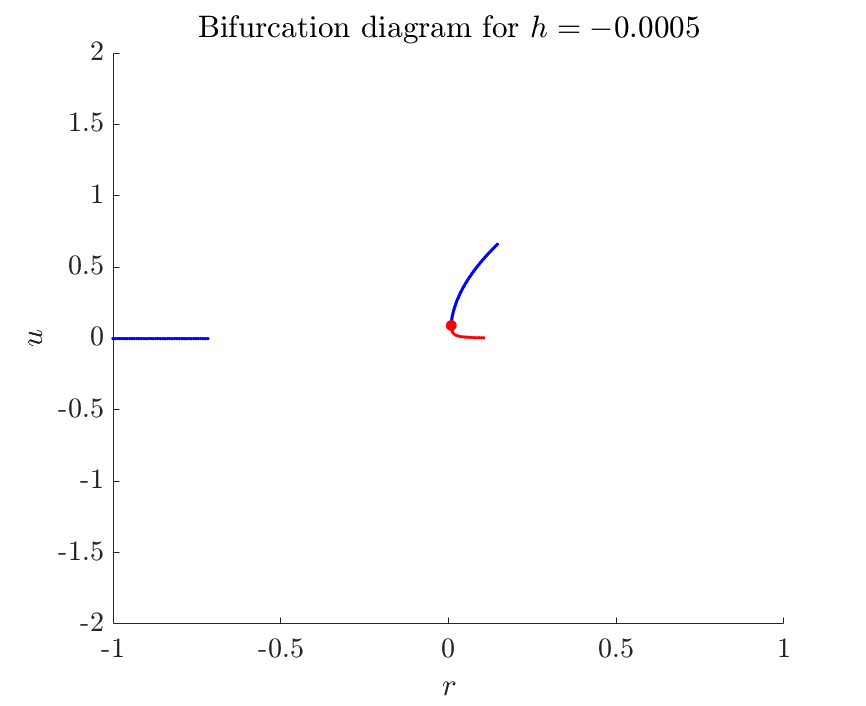
\includegraphics[width=\textwidth]{steps.png}
		\captionsetup{width=0.9\textwidth}
		\caption{Partially computed branches - too few continuation iterations (\texttt{cont - ItMX = 40}).}
		\label{fig:steps}
	\end{subfigure}
	}
	\caption{Bifurcation diagrams in function of $r$ for $h=-0.0005$ and $h=-0.0025$, obtained with \texttt{COCO}.}
\end{figure}
In both plots, the second part of the leftmost branch is lost. This shows why the right continuation parameters are so important.
\end{document}